

\newcommand{\comment}[1]{}
\newcommand{\myBigBreak}{\\[5mm]}
\newcommand{\vettore}[1]{$\vec{#1}$}

% DEFINIZIONE COLORI
\definecolor{LightYellow}{rgb}{1,1,0.80}
\definecolor{LightRed}{rgb}{1,0.80,0.80}

% TABELLA "ATTENZIONE"
\newcommand{\Attenzione}[1]{
    \newcolumntype{a}{>{\columncolor{LightRed}}l}
    
    \begin{table}[H]
    \begin{center}
    \begin{tabular}{|a|}
    \hline
     ATTENZIONE: \\
    \hline
    \end{tabular}
    \vspace{-4mm}
    
    \end{center}
    
    \newcolumntype{t}{>{\columncolor{LightRed}}l}
    
    \begin{center}\begin{tabular}{|t|}
    \hline
    #1\\
    \hline
    \end{tabular}\end{center}
    %\vspace{-4mm}
    \end{table}
}

% TABELLA "NOTA"
\newcommand{\myNOTE}[1]{
    \begin{table}[H]
    \newcolumntype{t}{>{\columncolor{LightYellow}}l}
    
    \begin{center}\begin{tabular}{|t|}
    \hline
    #1\\
    \hline
    \end{tabular}\end{center}
    %\vspace{-4mm}
    \end{table}
}

% DICHIARAZIONE myFOOTNOTES
\newcommand{\citIMU}{\nota{IMU: Inertial Measurement Unit}{}}
\newcommand{\citUART}{\nota{UART: Universal asynchronous receiver-transmitter}{}}
\newcommand{\citSPI}{\nota{SPI: Serial Peripheral Interface}{}}
\newcommand{\citItwoC}{\nota{I2C: Inter-Integrated Circuit}{}}
\newcommand{\citCPU}{\nota{CPU: Central Processing Unit}{}}
\newcommand{\citSRAM}{\nota{SRAM: Static Random-Access Memory}{}}
\newcommand{\citEEPROM}{\nota{EEPROM: Electronically Erasable Programmable Read-Only Memory}{}}
\newcommand{\citPWM}{\nota{PMW: Pulse-Width modulation}{}}

%%%%% Capitolo 1 %%%%%

\label{01-chapter}
In questo capitolo ho elencato\comment{registrato} i componenti principali utilizzati per il progetto, iniziando dalla scheda Arduino "Nano 33 BLE Sense" sulla quale caricherò come vedremo nel prossimo Capitolo un algoritmo di machine learning, proseguendo con la descrizione dei sensori di Hall, dei quali spiegherò la teoria alla base del loro funzionamento, ovvero "l'effetto Hall" da cui prendono il nome.\\
Infine darò una breve descrizione dell'applicativo web "Edge Impulse" [\riferimento{100-chapter}{1}], sul quale è possibile creare una rete neurale, allenarla e ricevere una libreria ZIP Arduino, contenente il modello della rete.

%Scheda Arduino utilizzata, riportando anche le sue specifiche.\\
%Sensore utilizzato e teoria dietro al suo funzionamento.\\
%Breve descrizione del sito "Edge Impulse"[\riferimento{100-chapter}{1}], utilizzato per l'addestramento della rete neurale e la creazione della libreria Arduino, utilizzata nel rispettivo codice.


\section{Arduino Nano 33 BLE Sense} \label{sezione 1-1}
L'Arduino Nano 33 BLE Sense è stata una delle prime schede sul mercato a supportare l'utilizzo dei modelli di machine learning costruiti con la libreria "TensorFlow Lite"[\riferimento{100-chapter}{2}]; sulla scheda di sviluppo sono inclusi anche vari sensori, che si possono trovare elencati nella relativa pagina ufficiale, [\riferimento{100-chapter}{3}] sul sito Arduino, con i relativi datasheet.\\
Possiamo utilizzarli direttamente nel codice Arduino, tramite l'Arduino IDE[\riferimento{100-chapter}{4}] ad esempio, installando le varie librerie, specifiche per ogni sensore.\\


\subsection{Esempio [Libreria LSM9DS1: Accelerometro]}
La libreria LSM9DS1 corrisponde all'accelerometro montato sull'Arduino, dopo averla installata tramite il gestore librerie dall'IDE, tramite il codice che vediamo qua sotto, è possibile scrivere sul monitor seriale i valori ottenuti dall'accelerometro.
\begin{lstlisting}[language=Arduino]
#include <Arduino_LSM9DS1.h>
void setup(){
    Serial.begin(115200);
    // Start accelerometer
    if (!IMU.begin()) {
        Serial.println("Failed to initialize IMU!");
        while (1);
    }
}//end setup

void loop(){
    float x, y, z
    IMU.readAcceleration(x, y, z);
}//end loop
\end{lstlisting}
\noindent\makebox[\linewidth]{\rule{15mm}{.4mm}}


\subsection{Lista dei sensori sulla board Arduino}
Come accennato in precedenza la scheda Arduino presenta dei sensori già saldati\comment{installati}\comment{montati}:
\begin{itemize}[noitemsep]
    \item{IMU\citIMU  [LSM9DS1]}
    \item{Microfono  [MP34DT05]}
    \item{Luce, Prossimità  [APDS9960]}
    \item{Pressione barometrica  [LPS22HB]}
    \item{Temperatura ed Umidità  [HTS221]}
\end{itemize}



\label{Figura 000.1}
\begin{figure}[H]
    \centering
    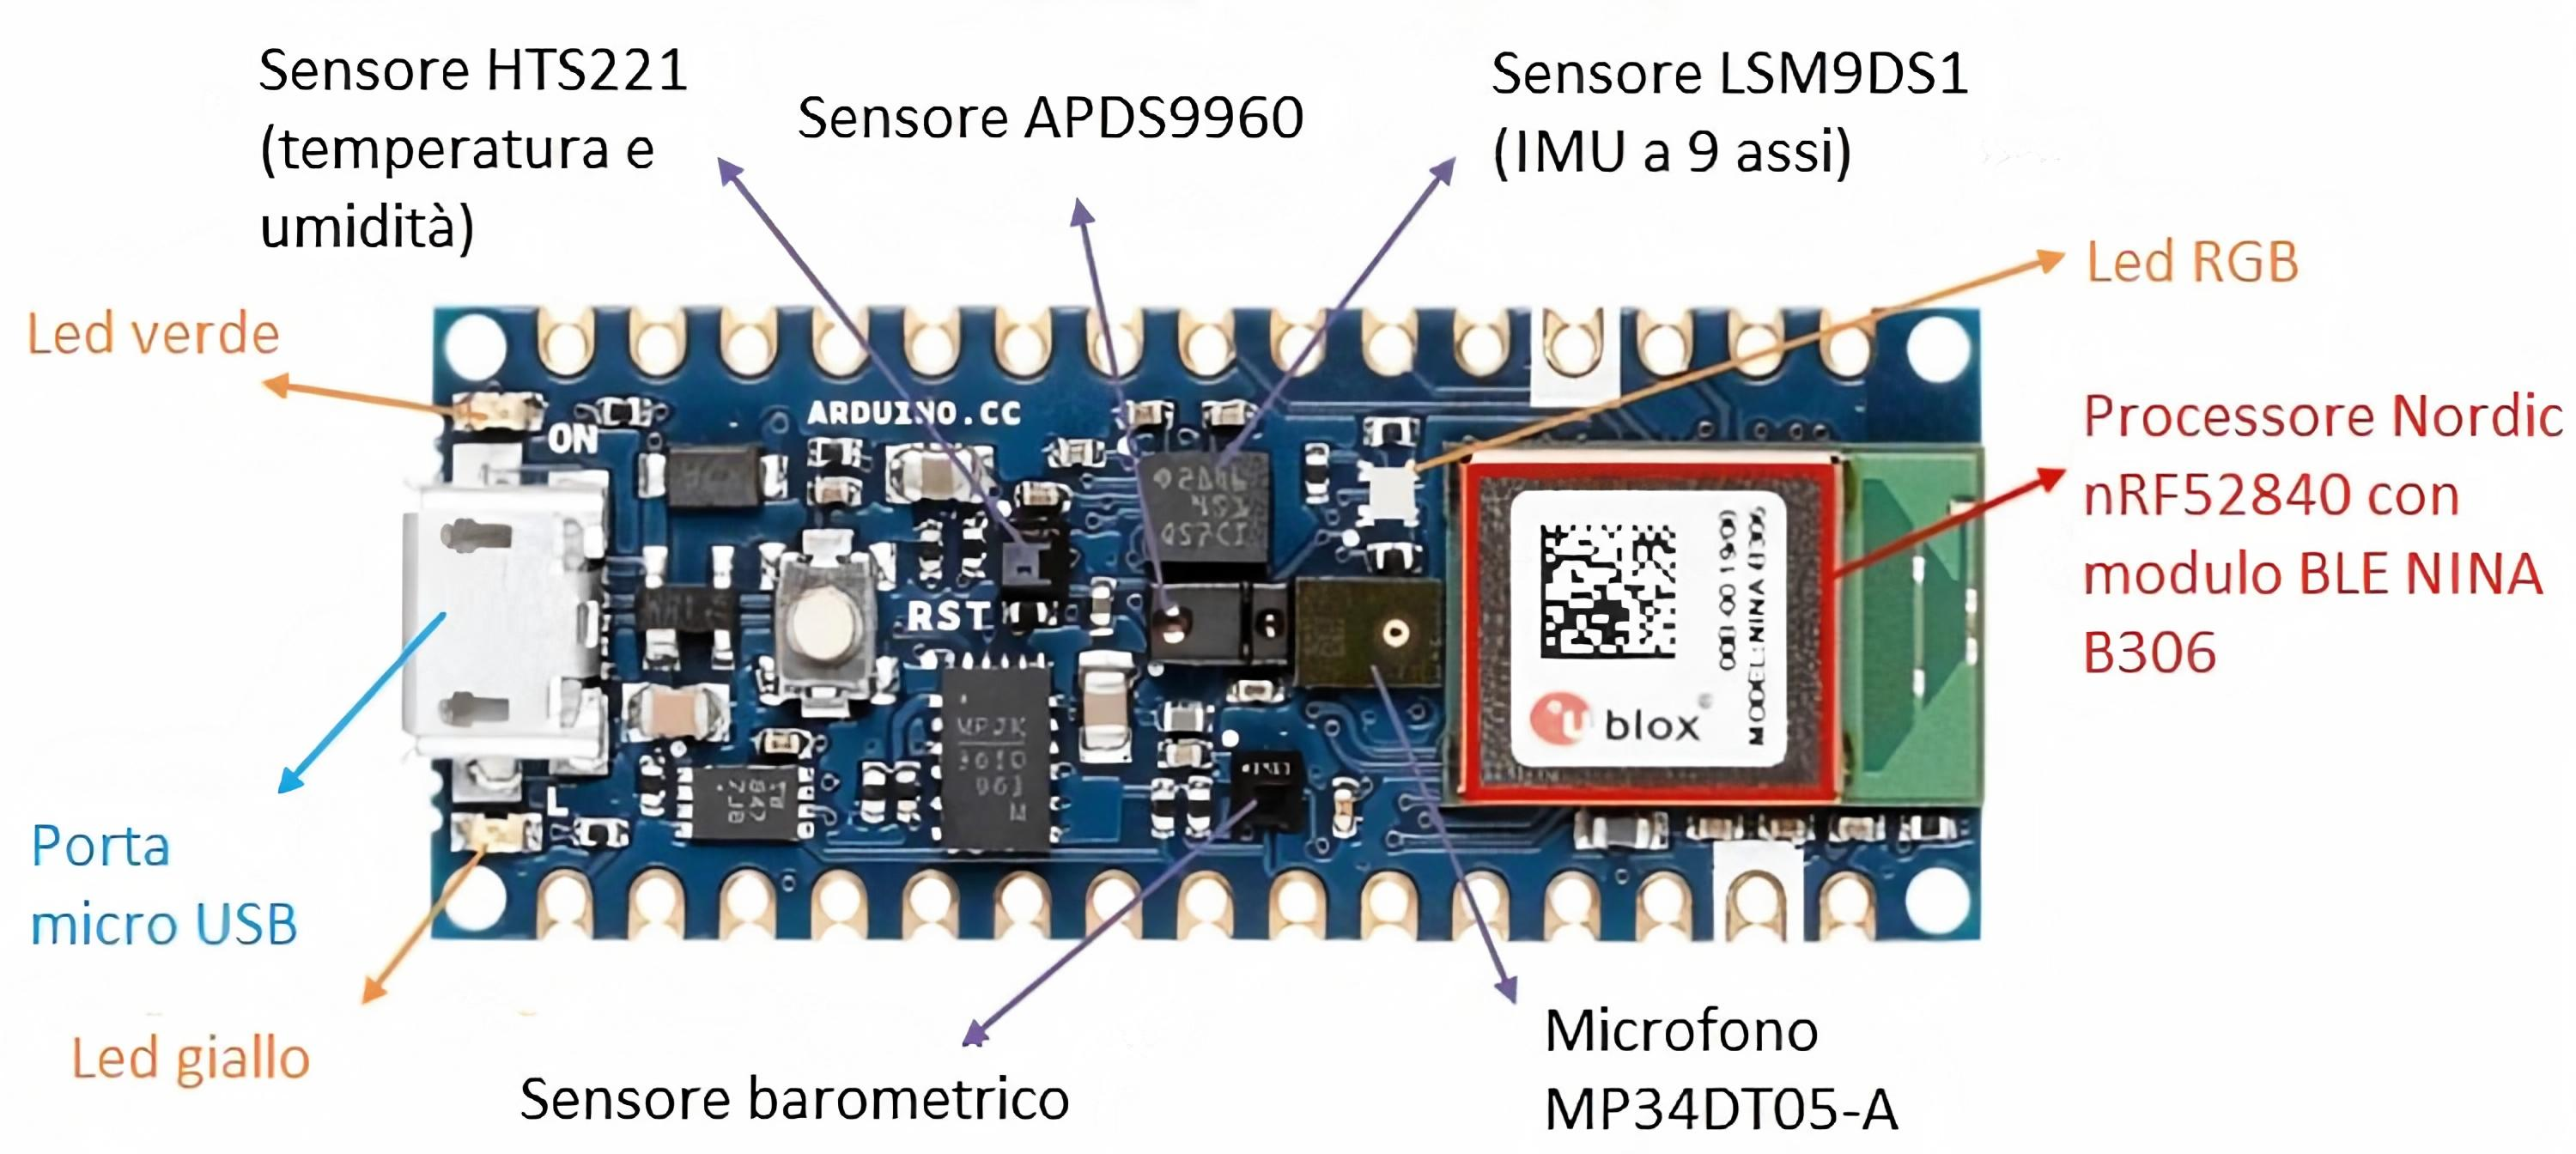
\includegraphics[width=\textwidth]{figures/Arduino_with_Sensors_4x.jpg}
    \caption{Scheda Arduino Nano 33 BLE - Nome e Posizione dei Componenti}
\end{figure}



\Attenzione{L'Arduino lavora a 3.3 V, di conseguenza accetta solamente voltaggi pari od inferiori a\\
\textbf{3.3 V}: se collegata a tensioni di valori superiori, la scheda potrebbe danneggiarsi}

\subsection{Specifiche Fondamentali della Scheda}
Di seguito ho riportato le informazioni ottenute\comment{prese}\comment{mostrate sulla} dalla pagina ufficiale sul sito Arduino, relative alla scheda di sviluppo: "Nano 33 BLE Sense"[\riferimento{100-chapter}{4}].\\
\begin{center} \begin{tabularx}{12,3cm}{|l l|}
\hline
    MICROCONTROLLER & nRF52840\\
    \hline
    OPERATING VOLTAGE & 3.3V\\
    INPUT VOLTAGE & 4.5V - 21V\\
    \hline
    DC CURRENT PER I/O PIN & 15 mA\\
    \hline
    CLOCK SPEED & 64MHz\\
    CPU\citCPU{} FLASH MEMORY & 1MB (nRF52840)\\
    SRAM\citSRAM{} & 256KB (nRF52840)\\
    EEPROM\citEEPROM{} & none\\
    \hline
    DIGITAL INPUT / OUTPUT PINS & 14\\
    PWM\citPWM{} PINS & all digital pins\\
    \hline
    UART\citUART{} & 1\\
    SPI\citSPI{} & 1\\
    I2C\citItwoC{} & 1\\
    \hline
    ANALOG INPUT PINS & 8 (ADC 12 bit 200 ksamples)\\
    ANALOG OUTPUT PINS & Only through PWM (no DAC)\\
    EXTERNAL INTERRUPTS & all digital pins\\
    \hline
    LED\_BUILTIN & 13\\
    \hline
    USB	Native in the & nRF52840 Processor\\
    \hline
\end{tabularx} \end{center}

\newpage{}


\section{Effetto Hall}\label{sezione 1-2}
L'effetto Hall è un fenomeno legato al passaggio di una corrente \textit{I} attraverso un conduttore, in una zona in cui è presente un campo magnetico, tramite questo fenomeno è possibile determinare due importanti caratteristiche del conduttore in questione: il segno dei portatori di carica e la loro densità [\riferimento{100-chapter}{5}].\\
Prende il nome dal fisico statunitense Edwin Hall, colui che ha scoperto questo effetto nel 1879 [\riferimento{100-chapter}{6}].\\
Indichiamo con \vettore{I} e \vettore{J} i due vettori che descrivono la corrente e la densità di corrente, rispettivamente, il cui verso è definito come: il verso in cui scorrerebbe la corrente, se i portatori di carica fossero positivi [\riferimento{100-chapter}{5}].\\
Rispetto alla velocità \vettore{v} dei portatori di carica, se questi ultimi sono portatori di carica positivi, allora \vettore{v} e \vettore{J} saranno paralleli; se invece i portatori di carica sono negativi i due vettori saranno antiparalleli [\riferimento{100-chapter}{5}].\\[7mm]

\label{IMAGE - Lastra di Metallo Sottoposta a corrente}
\begin{figure}[H]
    \centering
    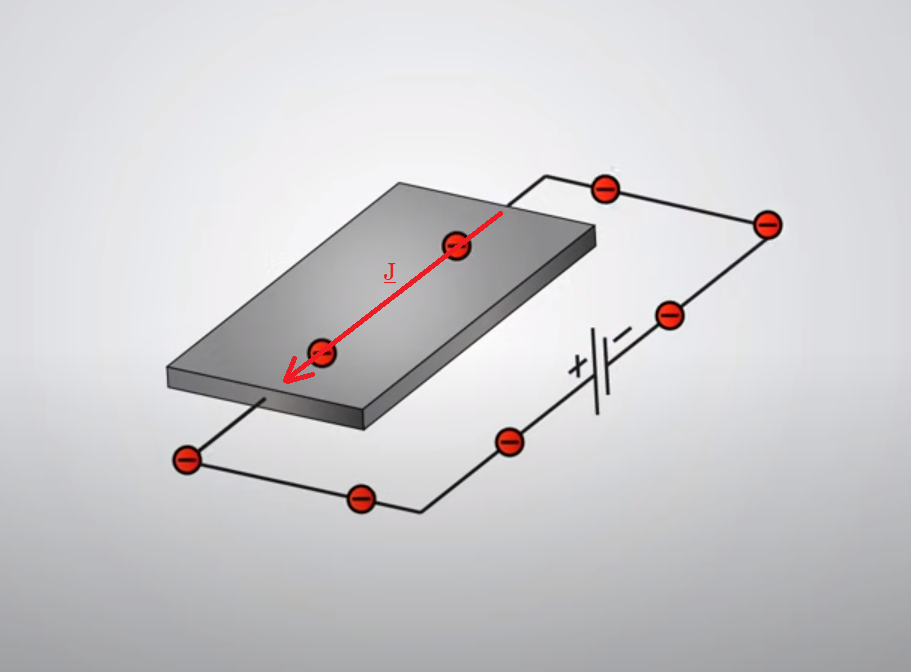
\includegraphics[width=\textwidth]{figures/Lastra di Metallo Sottoposta a corrente - Copia.PNG}
    \caption{Scorrimento di una corrente elettrica in una lastra di metallo}
\end{figure}

Supponiamo di avere un conduttore largo e sottile di superficie $S$, spessore $d$, \comment{e lo sottoponiamo} sottoposto ad un passaggio di corrente \vettore{I}, a cui corrisponde densità di corrente \vettore{J}, come illustrato in \riferimento{IMAGE - Lastra di Metallo Sottoposta a corrente}{Figura 1.2}.



Adesso si ipotizzi che la lastra di metallo sia soggetta ad un campo magnetico $\vec{B}$, come in \riferimento{IMAGE - Effetto della forza di Lorentz}{Figura 1.3}: tale campo modificherà il normale percorso della corrente, imponendogli una forza, in funzione del campo magnetico, detta "Forza di Lorentz".\\

\label{IMAGE - Effetto della forza di Lorentz}
\begin{figure}[H]
    \centering
    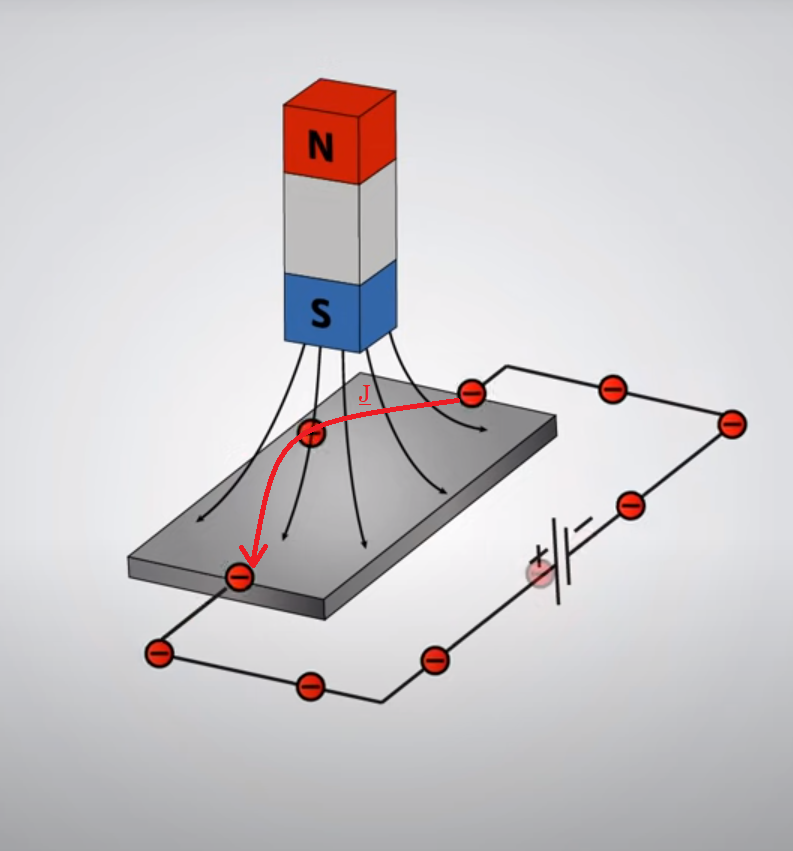
\includegraphics[width=145mm]{figures/Effetto_Hall_0 - Copia.PNG}
    \caption{Effetto della forza di Lorentz}
\end{figure}

Quindi, su ciascun portatore la forza impressa è:
\begin{equation} \label{eqn-1.1}
	\vec{F} = q\vec{v} \times{} \vec{B}
\end{equation}



In definitiva, a prescindere dal segno dei portatori di carica, ossia a prescindere
dal verso effettivo della corrente, l'azione del campo magnetico è sempre quella di
spingere trasversalmente (rispetto alla direzione della corrente) i portatori di carica,
addensandoli su un bordo del conduttore, come rappresentato in \riferimento{IMAGE - Misurazione dell'effetto Hall}{Figura 1.4}, portando così ad avere una differenza di potenziale $\Delta{}\varphi{}$ tra i bordi opposti del conduttore, che può essere misurata.\\
Basta allora stabilire il segno di questa differenza di potenziale per stabilire il segno dei portatori di carica.\\
La presenza di questa differenza di potenziale trasversale nei conduttori percorsi da corrente e soggetti ad un campo magnetico ad essa ortogonale, prende appunto il nome di "effetto Hall".[\riferimento{100-chapter}{5}].\\

\label{IMAGE - Misurazione dell'effetto Hall}
\begin{figure}[H]
    \centering
    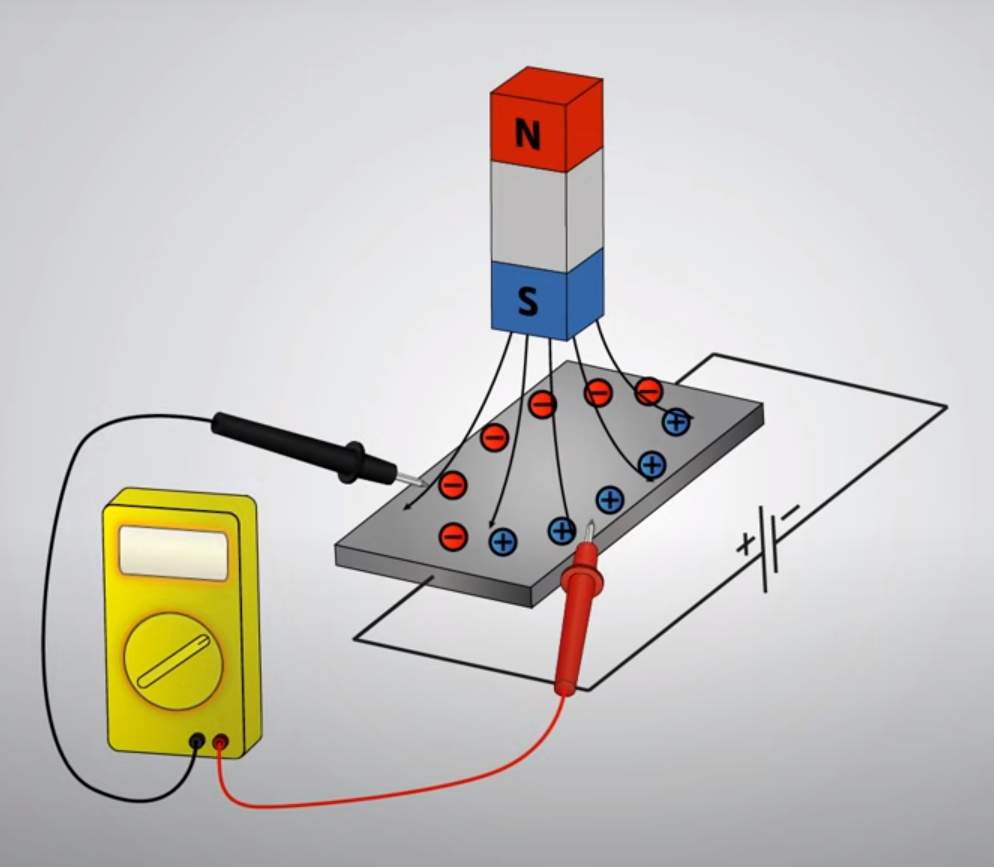
\includegraphics[width=\textwidth]{figures/Hall_effect_2.PNG}
    \caption{Misurazione dell'effetto Hall}
\end{figure}

\newpage{}

Il fatto che la forza di Lorentz faccia accumulare i portatori di carica su un bordo del conduttore, con conseguente creazione di una differenza di potenziale tra i due bordi opposti del conduttore, fa sì che si crei un campo elettrico \vettore{E_h} trasversale, diretto cioè ortogonalmente alla direzione della corrente. \\
Di conseguenza, quanta più corrente scorre, tanti più portatori vengono spinti dalla forza di Lorentz, e tanto maggiore sarà il valore di \vettore{E_h}; quindi se scorre più corrente, maggiore sarà la forza \vettore{F_h} che il campo elettrico trasversale esercita sugli stessi portatori [\riferimento{100-chapter}{5}].\\

\subsection{Differenza di potenziale data dall'effetto Hall}

Ricordiamo che comunque la forza elettrica \vettore{F_h} si oppone sempre alla forza magnetica, quindi, a prescindere dal segno dei portatori di carica, arriverà un momento in cui le due forze si equilibrano perfettamente,
cioè quando la forza di Lorentz risulta nulla:[\riferimento{100-chapter}{5}].

\begin{equation} \label{eqn-1.2}
	\vec{F} = q\vec{v} \times{} \vec{B} + q\vec{E_h} = 0
\end{equation}

Ricavando il valore del campo elettrico $\vec{E_h}$, all’equilibrio:
\begin{equation} \label{eqn-1.3}
	\vec{E_h} = -\vec{v} \times{} \vec{B}
\end{equation}

La velocità da considerare deve essere quella media dei portatori di carica, per
cui la relazione diventa:
\begin{equation} \label{eqn-1.4}
	\vec{E_h} = -\langle{}\vec{v}\rangle{} \times{} \vec{B}
\end{equation}

Indichiamo con N il numero totale di portatori di carica per unità di volume, possiamo quindi ricavare la densità di corrente:
\begin{equation} \label{eqn-1.5}
	\vec{J} = Nq\langle{}\vec{v}\rangle{}
\end{equation}

Da cui ricaviamo che:
\begin{equation} \label{eqn-1.6}
	\langle{}\vec{v}\rangle{} = \frac{\vec{J}}{Nq}
\end{equation}

Sostituendo nell’espressione del campo elettrico (1.4) , otteniamo:
\begin{equation} \label{eqn-1.7}
	\vec{E_h} = -\frac{1}{Nq} \cdot{} (\vec{J}\times{}\vec{B})
\end{equation}

Per definizione, la densità di corrente che scorre lungo il conduttore è data, in
modulo, dal rapporto tra la corrente $I$, e l’area $S$ del conduttore attraversata dalla
corrente stessa: considerando che abbiamo definito il conduttore con uno spessore $d$ e e larghezza $l$,\\ si deduce che: \comment{[\riferimento{100-chapter}{5}]}
\begin{equation} \label{eqn-1.9}
	S = d\cdot{}
\end{equation}
per cui: \\
\begin{equation} \label{eqn-1.9}
	J = \frac{I}{d\cdot{}}
\end{equation}

Sostituendo nella espressione del campo elettrico (1.7) e calcolando il modulo di tale campo, abbiamo:
\begin{equation} \label{eqn-1.8}
	\vec{E_h} = -\frac{J\cdot{}B}{Nq}sin\theta{} = -\frac{I\cdot{}B}{Nq\cdot{}d\cdot{}l}sin\theta{}
\end{equation}

Dove con $\theta{}$ viene indicato l’angolo formato dai vettori $\vec{J}$ e $\vec{B}$.\\
Se consideriamo $\theta{} = \pi{}/2$, ipotizzando che il campo \vettore{B} sia ortogonale alla direzione della corrente, avremo che il modulo del campo elettrico trasversale è:
\begin{equation} \label{eqn-1.9}
	\vec{E_h} = -\frac{I\cdot{}B}{Nq\cdot{}d\cdot{}l}sin\theta{} 
\end{equation}

Dal valore del campo all’equilibrio, si può risalire al valore della differenza di
potenziale \vettore{V_h} all’equilibrio:
\begin{equation} \label{eqn-1.10}
	\vec{V_h} = -\vec{E_h}\cdot{}l =  -\frac{I\cdot{}B}{Nq\cdot{}d}sin\theta{} 
\end{equation}

\myNOTE{
Si deduce che, a parità di forma del conduttore e a parità di campo magnetico, la\\
differenza di potenziale che si manifesta ai bordi del conduttore (una volta raggiunto\\
l’equilibrio) cresce proporzionalmente al crescere di $\vec{I}$, ed al diminuire del fattore $N\cdot{}q$,\\
che è appunto la densità spaziale di carica e che si può ricavare dalla relazione (1.11) [\riferimento{100-chapter}{5}].
}

\comment{ %Dont know if this figure is usefull or not
\label{}
\begin{figure}[H]
    \centering
    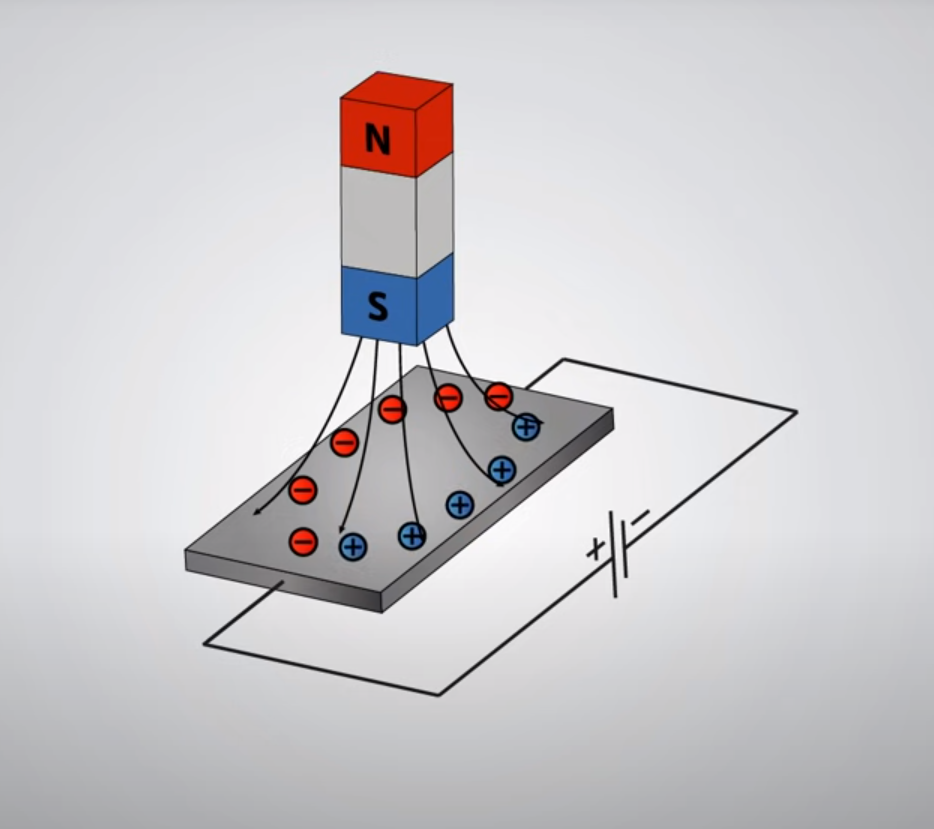
\includegraphics[width=\textwidth]{figures/Effetto Hall 1.PNG}
    \caption{}
\end{figure}
}

\newpage{}

\section{Sensori ad Effetto Hall}\label{sezione 1-3}
La famiglia A130 (A1301 e A1302) è composta da\comment{comprende} sensori \comment{a tempo continuo,}raziometrici lineari che sfruttano l'effetto Hall per fornire in uscita una tensione proporzionale al campo magnetico applicato.
\comment{Entrambi i dispositivi hanno una tensione in uscita a riposo,\comment{ovvero}\comment{in assenza di un campo magnetico} definita come la tensione in uscita in assenza di campo magnetico , pari al 50\% della tensione di alimentazione.}\\
Tutti i dispositivi appartenenti alla famiglia A130, in assenza di\comment{non soggetti ad} un campo magnetico significativo, presentano in uscita una tensione così detta "a riposo", pari al\comment{definita come il } 50\% della tensione di alimentazione.
Lo specifico sensore che andremo ad utilizzare (A1301) ha una sensibilità tipica pari ad $1.3$ $\mathrm{\frac{mV}{G}}$ [\riferimento{100-chapter}{7}].\\

Il circuito integrato ad effetto Hall, presente in ogni sensore, include un sensore di Hall, un amplificatore lineare ed una struttura CMOS di Classe A come stadio di uscita, lo schema a blocchi del sensore è riportato in \riferimento{IMAGE - Functional Block Diagram}{Figura 1.5}.\\
Integrare il sensore di Hall e l’amplificatore su un unico chip minimizza molti dei problemi normalmente associati a segnali analogici a basso livello di tensione [\riferimento{100-chapter}{7}].\\
Un’alta precisione nei livelli di uscita, viene inoltre ottenuta grazie ad una regolazione dell’offset, effettuata come ultimo passo del processo di produzione\comment{effettuata come ultimo passaggio, durante il processo di produzione} [\riferimento{100-chapter}{7}].\\

\label{IMAGE - Functional Block Diagram}
\begin{figure}[H]
    \centering
    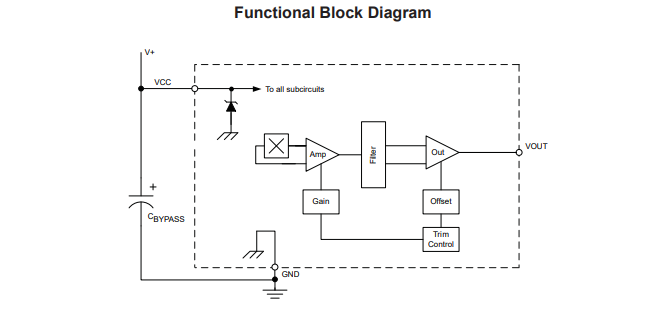
\includegraphics[width=\textwidth]{figures/Functional Block Diagram.PNG}
    \caption{Sensore ad effetto Hall A1302 - Functional Block Diagram}
\end{figure}

\label{IMAGE - Datasheet}
\begin{figure}[H]
    \centering
    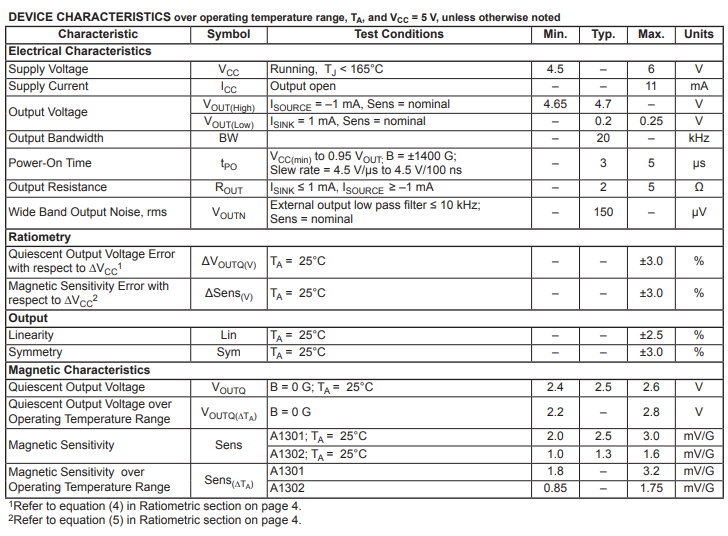
\includegraphics[width=135mm]{figures/Datasheet.PNG}
    \caption{Sensore ad effetto Hall A1302 - Datasheet}
\end{figure}

\label{IMAGE - Pin Out Drawings}
\begin{figure}[H]
    \centering
    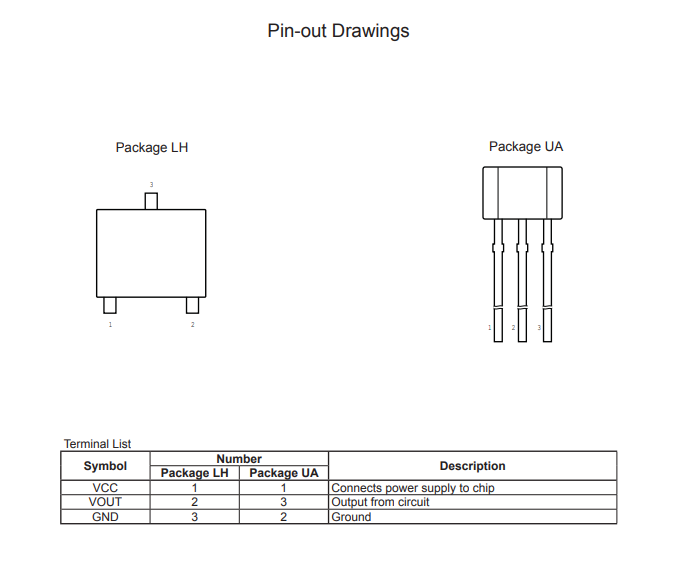
\includegraphics[width=125mm]{figures/Pin Out Drawings.PNG}
    \caption{Sensore ad effetto Hall A1302 - Pin Out Drawings}
\end{figure}

Come possiamo vedere in \riferimento{IMAGE - Functional Block Diagram}{Figura 1.7} sono disponibili due tipi di package per lo stesso dispositivo: LH, a 3-pin SOT23W specifico per il montaggio superficiale, ed il pacchetto UA, a 3-pin ultramini SIP per il montaggio a foro passante.\\
Entrambi i pacchatti sono senza piombo (Pb) ed i leadframes sono completamente placcati in stagno opaco\comment{ matte tin plated leadframes}.

\label{IMAGE - vs. Suplly Voltage}
\begin{figure}[H]
    \centering
    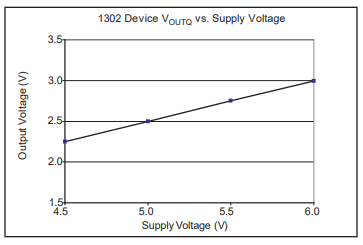
\includegraphics[width=75mm]{figures/Device Voutq vs. Supply Voltage.PNG}
    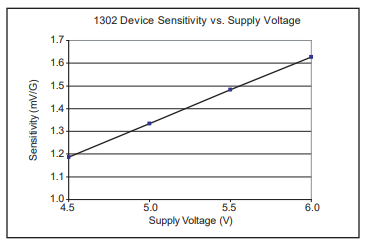
\includegraphics[width=75mm]{figures/Device Sensitivity vs. Supply Voltage.PNG}
    \caption{Sensore ad effetto Hall A1302 - Vout at Quiescent State and Sensitity vs. Supply Voltage}
\end{figure}

\textbf{Tensione in uscita a riposo}:\\
Quando il sensore si trova in uno stato di riposo (nessun campo magnetico significativo: \vettore{B}=0 T), in uscita $V_{outq}$ assume un valore pari a metà della tensione di alimentazione $V_{cc}$.
Data la temperatura ambiente $T_A$ ed il range della tensione di alimentazione $V_{cc}$, è possibile calcolare\comment{trovare} una tolleranza sulla tensione a riposo, $\Delta{}V_{outq}$, in funzione di $\Delta{}V_{cc}$ e $\Delta{}T_A$, viene definita come:
\begin{equation} \label{eqn-1.10}
	\Delta{}V_{outq}(\Delta{}T_A) = \frac{\Delta{}V_{outq}(T_A) - \Delta{}V_{outq}(25^{\circ{}})}{Sens(25^{\circ{}})}
\end{equation}
dove "$Sens$" si misura in $\mathrm{\frac{mV}{G}}$ ed \comment{il risultato assume il significato di}indica la sensitività del dispositivo\comment{il risultato finale espresso in Gauss (G), indica l'accuratezza del sensore, applicabile su tutto il range di temperatura}.\\

\textbf{Razionometrico}:\\
Il sensore A1301 è caratterizzato da un'uscita razionometrica, ciò vuol dire sia la $V_{outq}$, che la sensibilità magnetica, $Sens$, sono proporzionali alla tensione di alimentazione $V_{cc}$.
La percentuale di cambiamento (\%) della tensione in uscita a riposo è definita come:
\begin{equation} \label{eqn-1.10}
	\Delta{}V_{outq}(\Delta{}V) = \frac{V_{outq}(V_{cc}) / V_{outq}(5V)}{V_{cc} / 5V} \times{} 100\%
\end{equation}
Mentre il \textit{ratiometric change} (\%) per la Sensitività è definito come:
\begin{equation} \label{eqn-1.10}
	\Delta{}Sens(\Delta{}V) = \frac{Sens(V_{cc}) / Sens(5V)}{V_{cc} / 5V} \times{} 100\%
\end{equation}

\newpage{}

\textbf{Sensitività}:\\ 
La presenza di un campo magnetico a polarità positiva ($+{B}$), perpendicolare alla parte frontale del dispositivo, aumenta la tensione di uscita $V_{out}$, in proporzione al campo magnetico applicato, da $V_{outq}$ fino ad un massimo pari a $V_{cc}$.\\
Al contrario se si ha di fronte \comment{alla polarità negativa di campo magnetico}la polarità negativa di un campo magnetico ($-{B}$), nella stessa orientazione, ridurrà proporzionalmente $V_{out}$ da  $V_{outq}$ fino ad un minimo pari a 0 V.\\
La proporzionalità di queste variazioni è definita come la sensibilità magnetica del dispositivo:
\begin{equation} \label{eqn-1.10}
	Sens = \frac{V_{out}(-B) + V_{out}(+B)}{2B}
\end{equation}
La stabilità della sensibilità magnetica del dispositivo è una funzione della temperatura ambiente, $\Delta{}Sens(\Delta{}T_A)$ in percentuale (\%) è definita come:
\begin{equation} \label{eqn-1.10}
	\Delta{}Sens(\Delta{}T_A) = \frac{Sens(T_A) - Sens(25^{\circ{}})}{Sens(25^{\circ{}})} \times{} 100\%
\end{equation}

\textbf{Simmetria e Linearità}:\\
Lo stadio di uscita montato sul chip è costruito per fornire un'uscita lineare, se fornita una tensione di alimentazione pari a 5 V.\\
Anche se l'applicazione di forti campi magnetici non danneggiano il dispositivo, forzano però l'uscita in una zona di non-linearità.\\
La linearità in percentuale è misurata come segue:
\begin{equation} \label{eqn-1.10}
	Lin+ = \frac{V_{out}(+B) - V_{outq}}{2(V_{out}(+B\frac{1}{2}) - V_{outq})} \times{} 100\%
\end{equation}
\begin{equation} \label{eqn-1.10}
	Lin- = \frac{V_{out}(-B) - V_{outq}}{2(V_{out}(-B\frac{1}{2}) - V_{outq})} \times{} 100\%
\end{equation}
e la simmetria di uscita come:
\begin{equation} \label{eqn-1.10}
	Sym = \frac{V_{out}(+B) - V_{outq}}{V_{outq}) - V_{out}(-B)} \times{} 100\%\\[4mm]
\end{equation}

Riportate in \comment{questa scheda}questo paragrafo i grafici relativi alla tensione a riposo, ed alla sensibilità del dispositivo in rispetto alla tensione di alimentazione, in \riferimento{IMAGE - vs. Suplly Voltage}{Figura 1.8}, che saranno poi utili nell'utilizzo pratico del sensore[\riferimento{100-chapter}{7}].

\newpage{}

\section{Edge Impulse}\label{sezione 1-4}
Edge Impulse[\riferimento{100-chapter}{1}], ovvero TinyML come servizio, consente l'utilizzo dell'apprendimento automatico a tutti gli sviluppatori con un SDK (Software Development Kit) per dispositivi open source, sfruttando principalmente due librerie: "TensorFlow" per l'addestramento della rete neurale, e "TensorFlow Lite" per l'utilizzo su sistemi embedded.\\

Dalla pagina web è possibile: raccogliere dati da vari sensori, elaborare segnali in tempo reale, effettuare test \comment{e distribuire}su qualsiasi dispositivo\comment{supportato} [\riferimento{100-chapter}{8}].\\
%Gli SDK open source offerti da Edge Impulse consentono di raccogliere dati o distribuire codice su qualsiasi dispositivo [\riferimento{100-chapter}{8}].\\
In particolare viene offerta la possibilità di ottenere il modello di machine learning "TensorFlow Lite", dopo averlo addestrato, sia in un file di formato ".tflite", \comment{dopo averlo\comment{una volta} addestrato}come libreria Arduino (che vedremo in particolare nel prossimo Capitolo), \comment{ovviamente modificabile}oppure come libreria C++, Cube.MX CMSIS-PACK, WebAssembly o TensorRT.\\

Viene inoltre offerta la possibilità di inviare raccolte di dati tramite file con estensione:
\begin{itemize}[noitemsep]
    \item{".CBOR"}
    \item{".JSON"}
    \item{".CSV"}
    \item{".WAV" (per file audio)}
    \item{".JPG" (per immagini)}
    \item{".PNG" (per immagini)}\\
\end{itemize}

Edge Impulse è una piattaforma di sviluppo, gratuita per i singoli sviluppatori, che gli utenti possono contribuire ed estendere, aggiungendo e modificando algoritmi di machine learning, o implementando supporti per nuovi dispositivi. Il software del dispositivo, inclusi SDK, client, e codice generato, viene fornito come open source con una licenza Apache 2.0 [\riferimento{100-chapter}{8}].\\

